\chapter{基因组学与测序}\label{ch:b3:genomics}

第一个完整的自由生活生物基因组，即一种细菌的 \qty{1.8}{Mb}，
发表于 1995 年，由一支四十人的团队历时一年完成。
人类基因组含 32 亿个碱基对，
由一个国际联合体历时十三年、耗资约三十亿美元完成，
于 2003 年宣布竣工。
如今，一台台式机器一夜之间即可读完一个人的基因组，花费仅几百美元；
一家医院可对患者的肿瘤测序，以选择药物；
一家博物馆则能提取并读取一块四万年前骨骼的基因组。
使这一切成为可能的技术，
将数百万条短\omterm{def:b3:genomics:ngs}{读段}拼接成基因组的数学方法，
以及已完成的基因组所揭示的我们 DNA 的大小、内容与历史，
构成本章的主题。下一章讨论序列到手之后，
用于比较序列的算法。

\section{读取 DNA}

\begin{definition}[链终止测序]\label{def:b3:genomics:sanger}
\index{桑格测序}\index{双脱氧核苷酸}\index{链终止}
\emph{桑格测序}以单链为模板，从引物起始复制，
在 DNA 聚合酶作用下，于四种普通核苷酸和少量
\emph{双脱氧核苷酸}存在时进行；双脱氧核苷酸缺少 3$'$
羟基，故一旦掺入即终止链的延伸。
每种双脱氧核苷酸带有不同的荧光染料。
产物是一组片段的混合物，模板的每个位置各有一条，
每条片段都以已知种类的碱基结尾；在凝胶毛细管中按大小分离后，
片段依长度顺序经过检测器，
颜色的顺序即模板的序列。
一次运行可读取 \qtyrange{700}{900}{bp}，错误率低于 $10^{-3}$；
它仍是验证构建体或单个基因的方法。
\end{definition}

\begin{proof}[证据]
桑格、尼克伦和库尔森于 1977 年发表了该方法，并在同一年用它读取了
噬菌体 $\phi$X174 的 \qty{5386}{bp}——这是第一个完整的 DNA 基因组——
1981 年，他们又读取了人类线粒体的 \qty{16569}{bp}。
弗莱施曼及其同事（1995）读取了 \qty{1.83}{Mb} 的 \emph{Haemophilus influenzae}，
其做法是将整个基因组随机打断成片段，
对其中 \num{24000} 条进行测序，
再用计算机拼接\omterm{def:b3:genomics:ngs}{读段}，即\emph{全基因组鸟枪法}策略，
此后所有项目都在此基础上加以放大。
\end{proof}

\begin{omfigure}
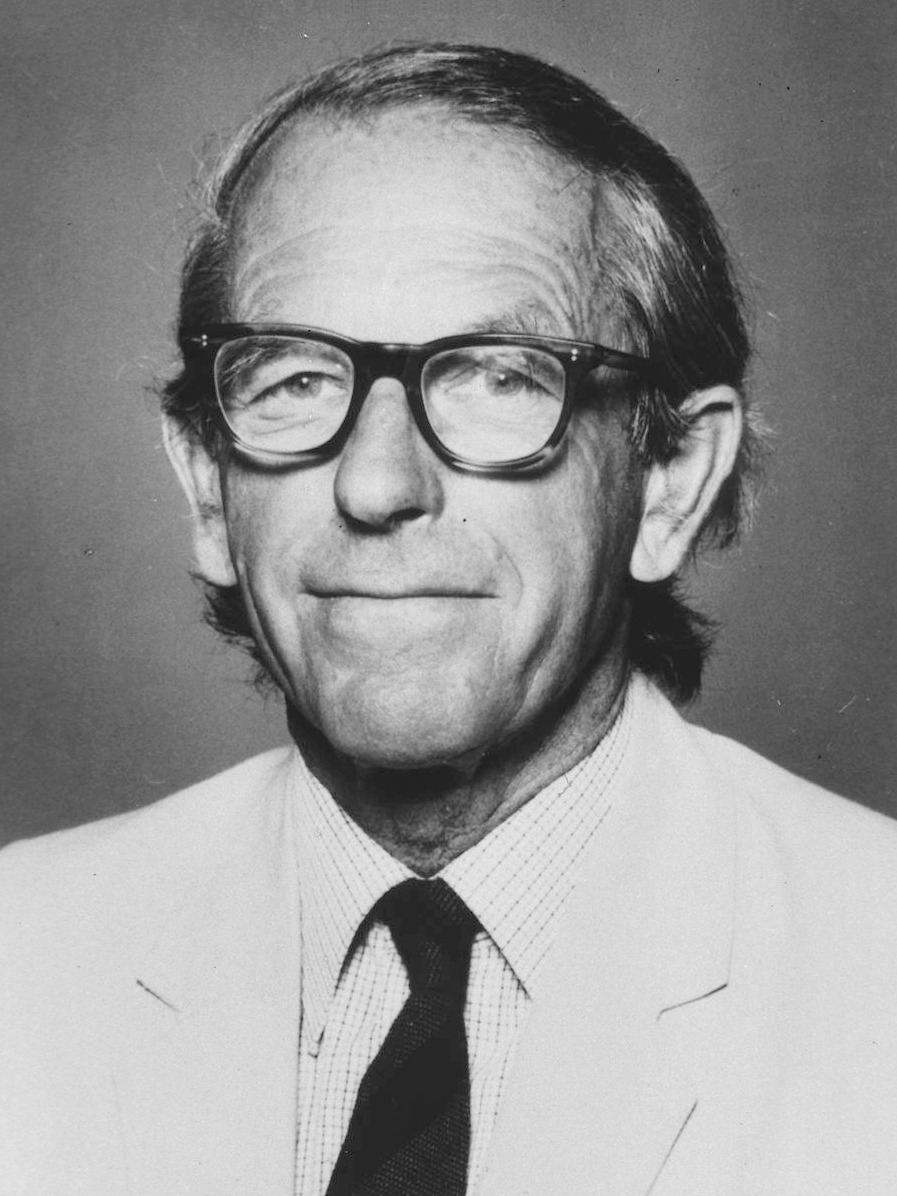
\includegraphics[width=0.30\linewidth]{images/book5/sanger.jpg}\hspace{0.04\linewidth}
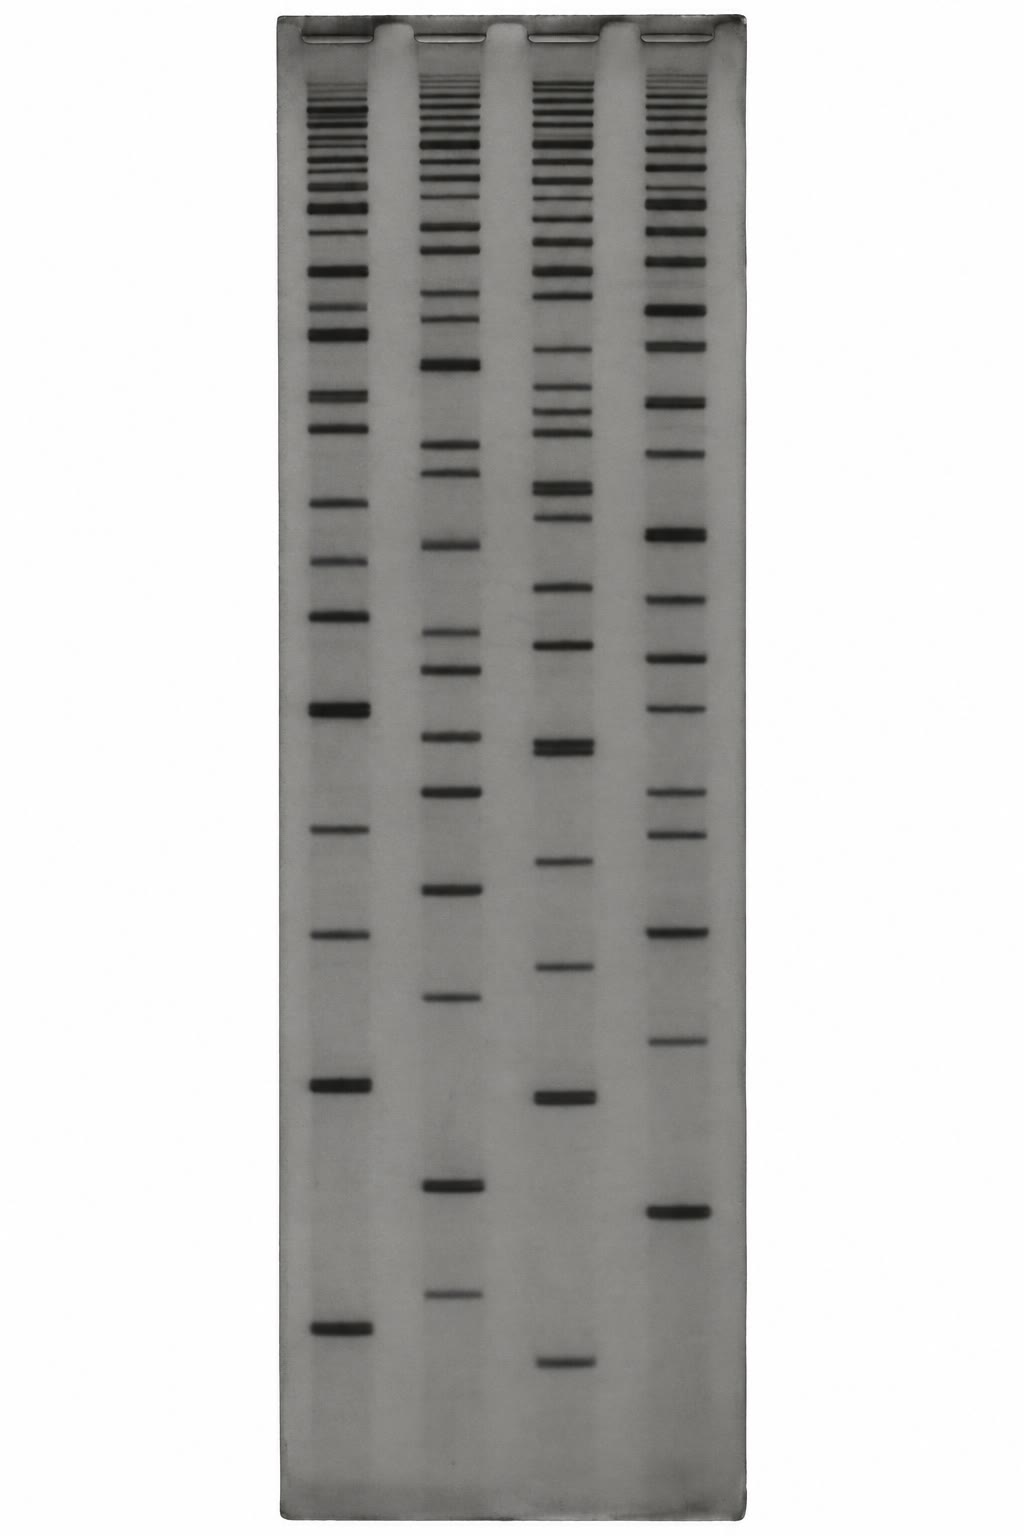
\includegraphics[width=0.30\linewidth]{images/book5/ai/b5-04-sanger-gel.jpg}

{\small 左：弗雷德里克·桑格，他设计了最早的实用蛋白质和 DNA 读取方法，两者均曾获诺贝尔奖。右：
毛细管时代之前测序凝胶的放射自显影片，
每条泳道对应一种碱基，
序列从梯状条带自下而上读出。}
\end{omfigure}

\begin{omfigure}
\begin{tikzpicture}[every node/.style={font=\scriptsize}, >=stealth]
  % template and primer
  \draw[very thick, omDef] (0,3.0) -- (6,3.0); \node[left] at (-0.1,3.0) {模板 3$'$};
  \node[right] at (6.05,3.0) {5$'$};
  \foreach \x/\b in {0.6/T,1.2/G,1.8/A,2.4/C,3.0/T,3.6/T,4.2/G,4.8/C} \node[above, omDef] at (\x,3.05) {\b};
  \draw[very thick, omProp] (0,2.6) -- (0.3,2.6); \node[left] at (-0.1,2.6) {引物};
  % terminated products
  \foreach \i/\len/\col/\b in {1/0.6/omDef/A, 2/1.2/omMeth/C, 3/1.8/omThm/T, 4/2.4/omExo/G, 5/3.0/omDef/A, 6/3.6/omDef/A, 7/4.2/omMeth/C, 8/4.8/omExo/G} {
    \draw[very thick, omProp] (0,2.6-0.32*\i) -- (\len-0.15,2.6-0.32*\i);
    \fill[\col] (\len-0.05,2.6-0.32*\i) circle (0.1);
    \node[right, \col] at (\len+0.05,2.6-0.32*\i) {dd\b};
  }
  \node[below, align=center] at (2.4,-0.25) {每个位置各有一条产物，末端为 \\荧光双脱氧碱基};
  % capillary readout
  \draw[->, thick] (6.5,1.3) -- (7.4,1.3) node[midway, above] {大小};
  \draw[thick] (7.6,0.0) rectangle (11.6,2.6);
  \foreach \i/\col in {1/omDef, 2/omMeth, 3/omThm, 4/omExo, 5/omDef, 6/omDef, 7/omMeth, 8/omExo} {
    \draw[very thick, \col] (7.6+0.45*\i,0.1) .. controls (7.6+0.45*\i-0.15,0.1) and (7.6+0.45*\i-0.1,1.6) .. (7.6+0.45*\i,1.6) .. controls (7.6+0.45*\i+0.1,1.6) and (7.6+0.45*\i+0.15,0.1) .. (7.6+0.45*\i+0.3,0.1);
  }
  \foreach \i/\b in {1/A, 2/C, 3/T, 4/G, 5/A, 6/A, 7/C, 8/G} \node[above] at (7.6+0.45*\i,1.7) {\b};
  \node[below] at (9.6,-0.05) {最短 $\to$ 最长：按颜色读出的序列};
\end{tikzpicture}

{\small \omterm{def:b3:genomics:sanger}{链终止}测序。双脱氧碱基在每个被掺入的位置终止复制；
每种长度各有一条片段，
片段按大小分离后，依次读取各末端碱基的颜色，
顺序即为序列。}
\end{omfigure}

\begin{definition}[大规模并行测序]\label{def:b3:genomics:ngs}
\index{边合成边测序}\index{读段}\index{长读长}\index{纳米孔}
第二代仪器可同时读取数百万至数十亿条片段。
在\emph{边合成边测序}中，片段两端连接接头后固定于玻璃流动槽上，
并在原位扩增为由相同分子组成的簇；
随后，每个循环以荧光且可逆封闭的核苷酸延伸一个碱基，
成像后去除封闭基团，再次延伸，
因此每个循环都为每个簇的\emph{读段}增加一个碱基。
读段长 \qtyrange{100}{300}{bp}，
通常从片段两端读取（\emph{双端}），
每个碱基的错误率约为 $10^{-3}$，
一次运行最多可产生 $10^{12}$ 个碱基。
第三代\emph{长读长}仪器无需扩增即可读取单分子：
一种方法是实时观察单个聚合酶掺入荧光核苷酸，
另一种方法是让 DNA 穿过蛋白质\emph{纳米孔}，并记录离子电流，
每种碱基序列以各自的方式调制该电流。
长达 \qtyrange{10}{100}{kb} 或更长的读段，
能够跨越短读段无法跨越的重复序列，
其原始错误率较高，但可通过一致序列加以降低。
\end{definition}

\begin{omfigure}
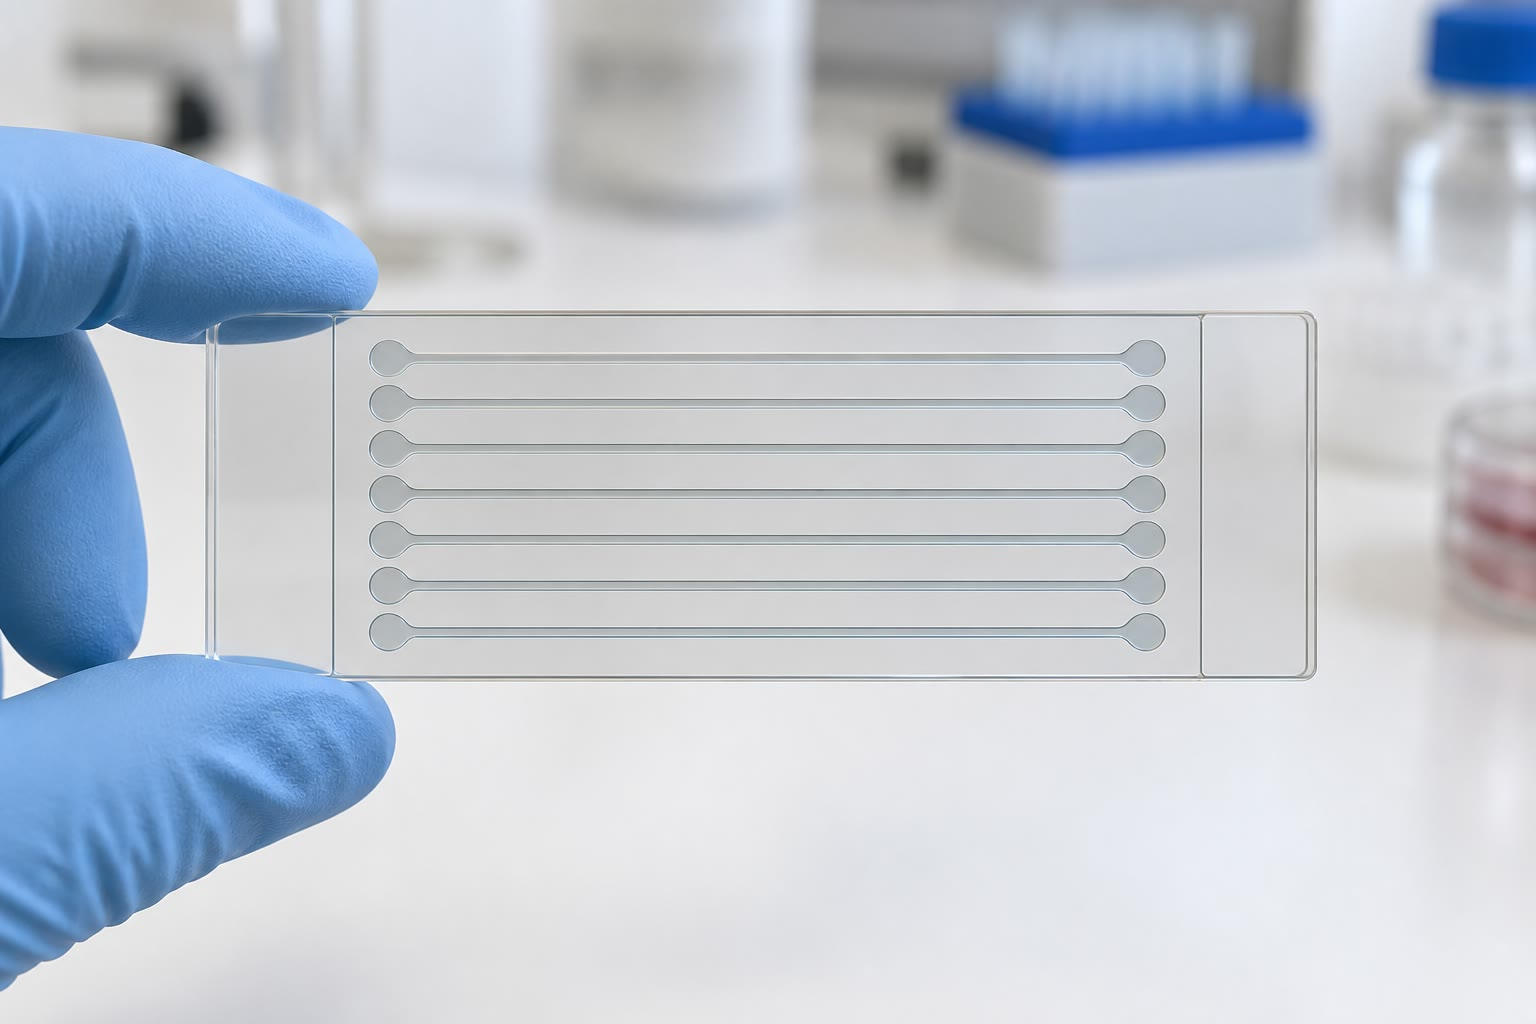
\includegraphics[width=0.46\linewidth]{images/book5/ai/b5-04-flowcell.jpg}\hspace{0.04\linewidth}
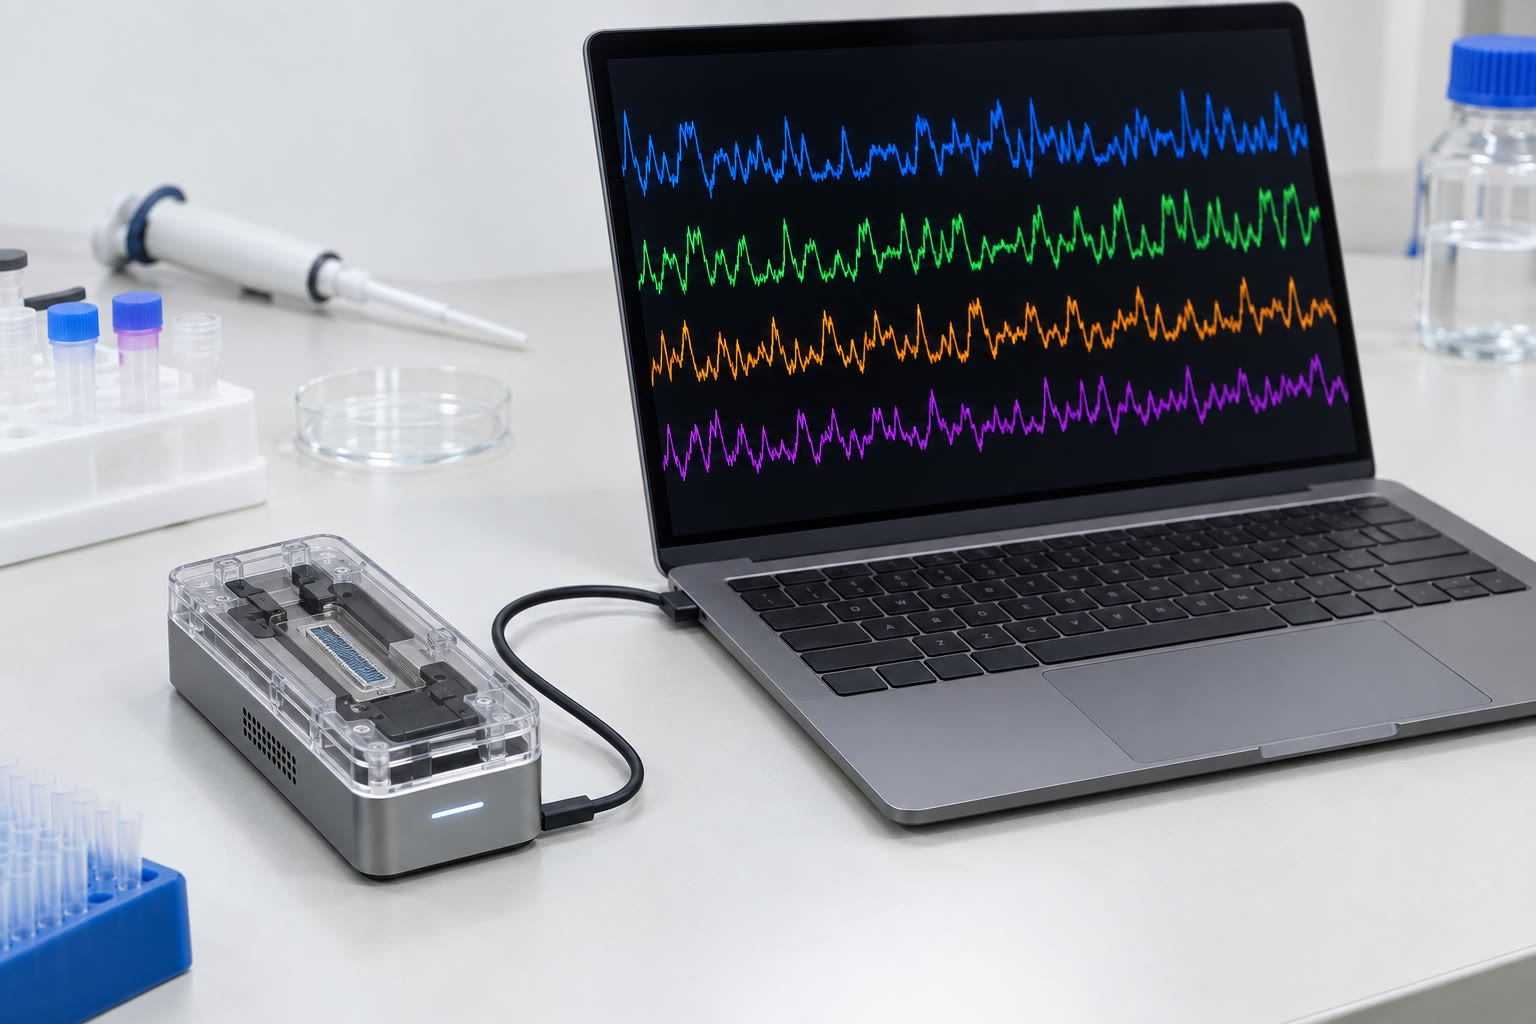
\includegraphics[width=0.46\linewidth]{images/book5/ai/b5-04-nanopore.jpg}

{\small 左：流动槽，即一块玻璃载片，上面生长出数十亿个 DNA 簇，
每个循环读取一个碱基。右：袖珍型\omterm{def:b3:genomics:ngs}{纳米孔}测序仪，
以离子电流的变化读取单分子，
这些变化即为读数。}
\end{omfigure}

\begin{theorem}[鸟枪法测序项目中的覆盖度与空位]\label{thm:b3:genomics:lander-waterman}
\index{覆盖度}\index{兰德–沃特曼}\index{重叠群}
设随机选取 $N$ 条长度为 $L$ 的\omterm{def:b3:genomics:ngs}{读段}，其位置沿长度为
$G$ 的基因组随机分布，令 $c = NL/G$ 为\emph{覆盖度}，即
覆盖某一碱基的\omterm{def:b3:genomics:ngs}{读段}平均数。于是任一给定碱基被
覆盖的\omterm{def:b3:genomics:ngs}{读段}数服从均值为 $c$ 的泊松分布，未测序部分
占基因组的比例为
\[
P(\text{未覆盖}) = e^{-c},
\]
若两条\omterm{def:b3:genomics:ngs}{读段}仅当共享的碱基数至少为
$T$ 个时才被识别为重叠，记 $\theta = T/L$，则期望的
\emph{重叠群}（由重叠\omterm{def:b3:genomics:ngs}{读段}构成的“岛”）数目为
\[
\text{重叠群} = N\,e^{-c(1-\theta)},
\]
其平均长度为 $L\,\bigl(e^{c(1-\theta)} - 1\bigr)/c + L\theta$，
（近似）。
\end{theorem}
\begin{proof}
\omterm{def:b3:genomics:ngs}{读段}起点随机出现，每个碱基处的起点密度为 $N/G$。一个碱基
被其前 $L$ 个碱基之内起点的\omterm{def:b3:genomics:ngs}{读段}所覆盖；此窗口长度为 $L$ 时起点数
服从均值为 $LN/G
= c$ 的泊松分布，无起点的概率为 $e^{-c}$。一个\omterm{def:b3:genomics:ngs}{读段}是其重叠群中最右的\omterm{def:b3:genomics:ngs}{读段}，
当且仅当其起点之后 $L - T = L(1-\theta)$ 个碱基内无其他\omterm{def:b3:genomics:ngs}{读段}起点
（起点更靠后的\omterm{def:b3:genomics:ngs}{读段}与之重叠的碱基数
少于 $T$ 且不被连接）；该概率为 $e^{-c(1-\theta)}$，
由于每个重叠群恰有一个最右\omterm{def:b3:genomics:ngs}{读段}，故期望数目
为 $N e^{-c(1-\theta)}$。平均重叠群长度
由 $G$ 除以重叠群数目得出，
并对未覆盖部分作修正。
\end{proof}

\begin{example}[覆盖到何种程度才足够]\label{ex:b3:genomics:coverage}
当 $c = 5$ 时未测序比例为 $e^{-5} = 0.7\,\%$——对于一个
\qty{3.2}{Gb} 的基因组，约两千万个碱基分散在数万个
空位之中。当 $c = 10$ 时，比例为 $4.5\times 10^{-5}$，共计 \qty{150}{kb}。
人类基因组通常以 $c = 30$ 测序，原因并非
覆盖空位（$e^{-30} \approx 10^{-13}$），而是因为每个碱基都须
在两条染色体上各被读取数次，以便
以可靠判定杂合变异，而单条\omterm{def:b3:genomics:ngs}{读段}的错误率为 $10^{-3}$。
细菌基因组的测序覆盖度为 $c = 50$--$100$，出于同样的原因
也因为成本低廉。该公式还说明了覆盖度无法弥补之处：
长于\omterm{def:b3:genomics:ngs}{读段}的重复序列即为
重叠图的分支点，无论多少短\omterm{def:b3:genomics:ngs}{读段}都无法将其分辨。这正是
长\omterm{def:b3:genomics:ngs}{读段}的用途所在。
\end{example}

\begin{omfigure}
\begin{tikzpicture}
\begin{axis}[
  width=0.7\linewidth, height=5.6cm,
  axis x line=bottom, axis y line=left,
  xmin=0, xmax=12, ymin=0.000001, ymax=1, ymode=log,
  xlabel={覆盖度 $c$}, ylabel={比例},
  xlabel style={font=\small, at={(axis description cs:0.5,-0.12)}, anchor=north},
  ylabel style={font=\small},
  tick label style={font=\small}, xtick={0,2,4,6,8,10,12},
  clip=false,
]
\addplot[very thick, omDef, domain=0:12, samples=40] {exp(-x)};
\addplot[very thick, omThm, domain=0.3:12, samples=40] {exp(-x*0.8)*x/12};
\node[font=\scriptsize, omDef, anchor=north west] at (axis cs:0.3,0.002) {未覆盖比例 $e^{-c}$};
\node[font=\scriptsize, omThm, anchor=south west] at (axis cs:5.5,0.03) {每条读段的重叠群数 $\times\, c/12$, $\theta = 0.2$};
\end{axis}
\end{tikzpicture}

{\small \omterm{thm:b3:genomics:lander-waterman}{兰德–沃特曼}两个量随覆盖度变化：
未被读取的基因组比例随 $e^{-c}$ 下降，而
重叠群数（此处按每条\omterm{def:b3:genomics:ngs}{读段}计）在低覆盖度时达到峰值，之后
随“岛”合并而下降。}
\end{omfigure}

\section{从读段到基因组}

\begin{definition}[组装与注释]\label{def:b3:genomics:assembly}
\index{组装}\index{支架}\index{N50}\index{注释}\index{参考基因组}
\emph{组装}通过重叠关系由\omterm{def:b3:genomics:ngs}{读段}重建基因组：在
\emph{重叠图}中，每条\omterm{def:b3:genomics:ngs}{读段}为一个节点，与其重叠的\omterm{def:b3:genomics:ngs}{读段}相连；
在\emph{de Bruijn 图}中，适用于数十亿条短\omterm{def:b3:genomics:ngs}{读段}，
每个 $k$-mer（长度为 $k$ 的子序列）为一个节点，基因组
即为穿过这些节点的路径。二者均会被长于\omterm{def:b3:genomics:ngs}{读段}的重复序列打断，
进而产生分支路径。重叠群经排列与定向，
借助双端\omterm{def:b3:genomics:ngs}{读段}及长程信息构成\emph{支架}，
（长\omterm{def:b3:genomics:ngs}{读段}、光学图谱和染色体接触图谱），随后
将支架定位到染色体上。组装质量可由
\emph{N50} 概括，即一个重叠群长度，使得组装碱基中
有一半位于不短于该长度的重叠群中。\emph{注释}随后
寻找基因：在细菌中即寻找长于随机预期的开放阅读框；在真核生物中，
则综合序列信号（剪接位点、启动子、密码子偏好性）、
与已知蛋白质的同源性，以及由
RNA 测序得到的转录本。对某一物种而言，结果即为\emph{参考基因组}，
此后该物种的每条\omterm{def:b3:genomics:ngs}{读段}都比对到其上，
而不必重新组装。
\end{definition}

\begin{method}[从样本到变异]\label{met:b3:genomics:pipeline}
\index{变异检测}
针对某个体的重测序研究，以\omterm{def:b3:genomics:assembly}{参考基因组}为参照：（1）
提取 DNA，将其打断为 \qtyrange{300}{500}{bp} 的片段，并连接接头
（即\emph{文库}）；（2）按所需覆盖度测序（人类基因组为 30$\times$
，外显子组为 100$\times$，外显子组捕获的是
基因组中编码蛋白质的 \qty{1.5}{\%}）；（3）将每条
\omterm{def:b3:genomics:ngs}{读段}比对到\omterm{def:b3:genomics:assembly}{参考基因组}，允许错配；（4）在每个位置
统计\omterm{def:b3:genomics:ngs}{读段}中的碱基：若约半数\omterm{def:b3:genomics:ngs}{读段}与参考序列不一致的位置，
即为杂合\emph{变异}；若几乎全部不一致，
则为纯合变异；若仅少数不一致，则为错误；
（5）按深度、碱基质量及链平衡进行过滤；（6）为每个
变异对任一基因的效应（同义、错义、无义、
剪接、移码），并标注其在群体数据库中的频率；（7）
若用于诊断，则保留位于基因中、预测有害的稀有变异，
这些基因须与表型相符，并以\omterm{def:b3:genomics:sanger}{桑格测序}加以确认。
\end{method}

\section{基因组的面貌}

\begin{proposition}[基因组大小与基因数目]\label{prop:b3:genomics:sizes}
\index{C 值矛盾}\index{基因组大小}
真核生物的\omterm{prop:b3:genomics:sizes}{基因组大小}跨度可达 $10^{5}$ 倍——
酵母为 \qty{12}{Mb}，线虫为 \qty{100}{Mb}，
果蝇为 \qty{140}{Mb}，人类为 \qty{3.2}{Gb}，洋葱为 \qty{16}{Gb}，
肺鱼为 \qty{130}{Gb}，百合 \emph{Paris
japonica} 为 \qty{150}{Gb}——而基因数目的跨度仅约 $10$ 倍：
酵母约 \num{6000} 个，线虫约 \num{20000} 个，果蝇约 \num{14000} 个，
人类约 \num{20000} 个编码蛋白质的基因，水稻约 \num{40000} 个。
这就是\emph{C 值矛盾}：\omterm{prop:b3:genomics:sizes}{基因组大小}不能衡量复杂性，
基因数目同样不能。变化的是非编码部分——
内含子、转座元件、卫星重复序列——而
基因组所能产生的蛋白质种类，
经可变剪接（见\cref{ch:b3:rna-regulation}）与调控，远超其基因数目，
生物体的复杂性恰在于此，
主要由此体现。细菌基因组则相反，结构紧凑，其
大小确与基因数目相关：约每千碱基一个基因，
\emph{E.~coli} 中编码序列占 \qty{88}{\%}。
\end{proposition}

\begin{example}[按内容划分的人类基因组]\label{ex:b3:genomics:content}
在 \qty{3.2}{Gb} 中：编码蛋白质的外显子占 \qty{1.5}{\%}；
基因的内含子与非翻译区约占 \qty{35}{\%}；转座元件及其化石约占 \qty{45}{\%}——
其中 LINE-1 反转录转座子占 \qty{17}{\%}，
Alu 元件占 \qty{10}{\%}（超过一百万份
\qty{300}{bp} 序列的拷贝），内源性逆转录病毒占 \qty{8}{\%}；片段重复
占 \qty{5}{\%}；简单重复与卫星序列（包括
着丝粒），约占 \qty{5}{\%}；其余为独特的非编码序列，
调控元件即位于其中。约 \numrange{100}{200} 个基因
仍编码活跃的 LINE-1 机制，新的插入大约
每二十次出生中出现一次。基因组中约 \qty{8}{\%} 处于
可检测的纯化选择之下——远多于外显子所占比例——且
其中大部分是调控元件。
\end{example}

\begin{omfigure}
\begin{tikzpicture}[every node/.style={font=\scriptsize}]
  \def\w{12}
  % stacked bar: fractions
  \fill[omThm] (0,0) rectangle (0.18,0.7);
  \fill[omDef!60] (0.18,0) rectangle (4.38,0.7);
  \fill[omProp!70] (4.38,0) rectangle (6.42,0.7);
  \fill[omProp!45] (6.42,0) rectangle (7.62,0.7);
  \fill[omProp!25] (7.62,0) rectangle (9.78,0.7);
  \fill[omMeth!50] (9.78,0) rectangle (10.38,0.7);
  \fill[gray!45] (10.38,0) rectangle (10.98,0.7);
  \fill[gray!15] (10.98,0) rectangle (12,0.7);
  \draw[thick] (0,0) rectangle (12,0.7);
  % labels above/below with leaders
  \draw (0.09,0.7) -- (0.09,1.1); \node[above, align=center] at (0.5,1.1) {外显子 \\\qty{1.5}{\%}};
  \node[above] at (2.3,0.75) {基因内含子、UTR：\qty{35}{\%}};
  \node[below, align=center] at (5.4,-0.05) {LINE-1\\\qty{17}{\%}};
  \node[below, align=center] at (7.0,-0.05) {Alu 元件 \\\qty{10}{\%}};
  \node[below, align=center] at (8.7,-0.05) {其他转座子、\\逆转录病毒 \qty{18}{\%}};
  \node[above, align=center] at (10.1,0.75) {片段重复 \qty{5}{\%}};
  \node[below, align=center] at (10.7,-0.05) {卫星序列 \\\qty{5}{\%}};
  \draw[gray] (11.5,0.72) -- (12.0,1.05); \node[above, align=center] at (12.3,1.05) {其他独特 \\非编码};
  \draw[decorate, decoration={brace, amplitude=4pt, mirror}] (4.38,-1.0) -- (9.78,-1.0) node[midway, below=4pt] {转座元件来源：\qty{45}{\%}};
\end{tikzpicture}

{\small 按内容划分的人类基因组，按比例绘制。蛋白质编码外显子
（红色）仅占一小条；近一半的基因组来源于
转座元件。}
\end{omfigure}

\begin{definition}[比较基因组学]\label{def:b3:genomics:comparative}
\index{直系同源基因}\index{旁系同源基因}\index{共线性}\index{保守非编码元件}\index{全基因组复制}
两个物种中的基因若源于其共同祖先的同一个基因，
称为\emph{直系同源基因}；同一物种内源于
重复的基因称为\emph{旁系同源基因}。
在不同物种间基因顺序保守的染色体片段称为\emph{共线的}；共线性使
得以依据一个基因组中的位置，在另一基因组中定位同一基因，
并揭示区分两种核型的重排（人与小鼠之间约
\num{1000} 处）。跨越远缘物种保守的序列
却不编码蛋白质——\emph{保守非编码元件}，
其中一些在人与鱼之间超保守至碱基水平，
跨度超过 \qty{200}{bp}，大多为发育基因的增强子。\emph{全基因组
复制}曾深刻塑造了各谱系的历史：脊椎动物起源时发生了两轮
（哺乳动物有四个 Hox 基因簇，无脊椎动物仅一个），
鲑科鱼类的祖先发生了一次，酵母谱系发生了一次，
开花植物中则发生了多次；重复基因大多
在数千万年间丢失，残存者在功能上发生
分化。
\end{definition}

\begin{example}[人与黑猩猩]\label{ex:b3:genomics:chimp}
比对的单拷贝序列在人与黑猩猩之间有
\qty{1.2}{\%} 的碱基不同——约 3500 万个替换——
另有插入与缺失，合计又使各自基因组相差
\qty{3}{\%}。两个人之间约每一千个碱基有一处差异，
约 \numrange{400}{500} 万个位点，另有数千个
结构变异；两只黑猩猩之间的差异则更多，因为它们的种群历史上
长期更大。一个孩子约带有 \num{70} 个新
突变，既不见于父母任何一方，其中五分之四来自
父亲，且父亲年龄每增加一岁，该数目约增加两个——
这正是把\cref{ch:b3:dna-repair}中的计算应用于
精子发生中的大量分裂。
\end{example}

\section{基因组与性状}

\begin{definition}[全基因组关联]\label{def:b3:genomics:gwas}
\index{全基因组关联研究}\index{单核苷酸多态性}\index{多基因评分}
\emph{单核苷酸多态性}（SNP）是指某一位点上，
两种碱基在一个种群中各自出现的频率均至少为 \qty{1}{\%}；
人类中约有一千万个常见的此类位点。\emph{全基因组关联
研究}（GWAS）在数千名患病者与数千名未患病者中，对数十万个 SNP 进行基因分型，
并在每个 SNP 处检验某一等位基因在病例中
是否更为频繁。因为要进行一百万次
检验，结果只有低于显著性阈值才算数，
该阈值约为 $5\times 10^{-8}$（$0.05$ 除以一百万个
实际独立的检验）。关联的 SNP 只标示一个区域，
而非致病变异本身，因为邻近等位基因会一同遗传（连锁
不平衡），可跨越数万个碱基。对于大多数常见疾病，
相关等位基因各自只使风险改变数个百分点，且大多
位于调控序列中；将它们的合并效应，即对数千个
SNP 求和所得的\emph{多基因评分}，能解释一部分
遗传力，其预测风险的能力大致与家族史相当。
\end{definition}

\begin{remark}[基因组学已取得和尚未取得的成果]\label{rem:b3:genomics:delivered}
测序在单个基因效应很大的情形中起了决定性作用：
数千种孟德尔病已找到其致病基因，对一名病因未明的患儿进行外显子组测序，
约三分之一的病例可由此得到诊断。
癌症基因组揭示肿瘤携带哪些驱动因素，
以及哪些药物可能有效（\cref{ch:b3:cancer-biology}）；
病原体基因组可以逐株追踪疫情的传播（\cref{ch:b3:bacteriology}）；
古代基因组改写了人类史前史，
表明非洲以外的人群携带约 \qty{2}{\%} 的尼安德特人 DNA。
对于常见病——糖尿病、
心脏病、精神分裂症——基因组学发现了数量众多的微小效应，
但可阐明的机制寥寥，
而从基因组预测健康个体患病风险的前景依然有限。基因组是一份零件清单，
而这些零件如何相互作用的生物学机制，并不能直接从中读出。
\end{remark}

\section{练习}

\begin{exercise}[$\star$]\label{exo:b3:genomics:1}
说明为何\omterm{def:b3:genomics:sanger}{双脱氧核苷酸}会终止正在延伸的 DNA 链，
以及为何桑格反应中每种核苷酸
都必须同时含有正常形式和双脱氧形式。
\end{exercise}

\begin{exercise}[$\star$]\label{exo:b3:genomics:2}
一次测序运行产生 $4\times 10^{8}$ 对、
每条 $2\times \qty{150}{bp}$ 的双端\omterm{def:b3:genomics:ngs}{读段}。它对 \qty{3.2}{Gb} 的人类基因组、
以及对 \qty{5}{Mb} 的细菌基因组分别给出多大的覆盖度？
\end{exercise}

\begin{exercise}[$\star$]\label{exo:b3:genomics:3}
定义重叠群、\omterm{def:b3:genomics:assembly}{支架}和 \omterm{def:b3:genomics:assembly}{N50}。某\omterm{def:b3:genomics:assembly}{组装}结果总长 \qty{100}{Mb}，
含 10 个长 \qty{8}{Mb} 的重叠群和 \num{2000} 个长 \qty{10}{kb} 的重叠群，求其 \omterm{def:b3:genomics:assembly}{N50}。
\end{exercise}

\begin{exercise}[$\star$]\label{exo:b3:genomics:4}
举两个例子说明 C 值悖论，
并说明大型基因组中多余 DNA 主要由什么造成。
\end{exercise}

\begin{exercise}[$\star\star$]\label{exo:b3:genomics:5}
利用\cref{thm:b3:genomics:lander-waterman}，
求使未测序碱基数至多为百万分之一所需的覆盖度；并求在 $c = 8$、
读长 \qty{150}{bp}、最小重叠 \qty{30}{bp} 的条件下，
对一个 \qty{5}{Mb} 基因组所得重叠群的期望数目。
\end{exercise}

\begin{exercise}[$\star\star$]\label{exo:b3:genomics:6}
某杂合变异位点被 $30$ 条\omterm{def:b3:genomics:ngs}{读段}覆盖。
假设每条\omterm{def:b3:genomics:ngs}{读段}以概率 $1/2$ 显示任一等位基因，
求显示变异等位基因的\omterm{def:b3:genomics:ngs}{读段}少于 $8$ 条（因而该变异可能被误判为错误）的概率。
用均值为 $15$、标准差为 $\sqrt{7.5}$ 的正态近似计算。
为何 $30\times$ 是通行的测序深度标准？
\end{exercise}

\begin{exercise}[$\star\star$]\label{exo:b3:genomics:7}
某基因组中有一段长 \qty{6}{kb} 的重复序列，
共 \num{500} 个拷贝。说明为何由 \qty{150}{bp} \omterm{def:b3:genomics:ngs}{读段}\omterm{def:b3:genomics:assembly}{组装}会将其塌缩，
所得图形呈何种形状，以及需要多长的读长才能将其分辨。
\end{exercise}

\begin{exercise}[$\star\star$]\label{exo:b3:genomics:8}
两个人在每一千个碱基中有一个碱基不同。
他们的外显子组（\qty{48}{Mb} 的编码序列）
中共有多少个差异？若编码区差异中有三分之二为同义或良性，
其余改变蛋白质，
则一人相对另一人携带多少个改变蛋白质的变异？
\end{exercise}

\begin{exercise}[$\star\star$]\label{exo:b3:genomics:9}
一项\omterm{def:b3:genomics:gwas}{全基因组关联研究}检验了 $10^{6}$ 个 SNP，
阈值为 $p < 5\times 10^{-8}$。
若没有任何 SNP 真正相关，
预期会出现多少个假阳性？某 SNP 等位基因使一种发病率为 \qty{2}{\%} 的疾病的风险升至 \qty{2.3}{\%}。
试说明为何这样的效应在一千人的研究中无法检测、
对个体毫无用处，却仍可能指向某一机制。
\end{exercise}

\begin{exercise}[$\star\star\star$]\label{exo:b3:genomics:10}
细菌基因组约 \qty{88}{\%} 为编码序列，
人类基因组则为 \qty{1.5}{\%}。就二者的差异，
给出三个假说——群体遗传学的、
结构性的和调节性的——并针对每一假说，给出一条支持或削弱它的基因组观察。
\end{exercise}

\begin{exercise}[$\star\star\star$]\label{exo:b3:genomics:11}
推导混合两种不同长度\omterm{def:b3:genomics:ngs}{读段}时的 Lander–Waterman 重叠群数目：
设 $N_{1}$ 条长度为
$L_{1}$ 的短\omterm{def:b3:genomics:ngs}{读段}与 $N_{2}$ 条长度为 $L_{2}$ 的长\omterm{def:b3:genomics:ngs}{读段}，
重叠均按相同的最小值 $T$ 计算。
（若任一类\omterm{def:b3:genomics:ngs}{读段}都不在其自身长度减 $T$ 的范围内起始，
则将每条\omterm{def:b3:genomics:ngs}{读段}视为其重叠群的最右端。）
证明少量长\omterm{def:b3:genomics:ngs}{读段}比等量碱基的短\omterm{def:b3:genomics:ngs}{读段}更能显著减少重叠群数目。
\end{exercise}

\begin{exercise}[$\star\star\star$]\label{exo:b3:genomics:12}
哺乳动物的四个 Hox 基因簇被认为源自脊椎动物起源处的一个基因簇，
经历了两轮\omterm{def:b3:genomics:comparative}{全基因组复制}。
请说明该假说预测全基因组中\omterm{def:b3:genomics:comparative}{旁系同源基因}呈何种分布模式，
以及七鳃鳗和无脊椎动物脊索动物的基因组中呈何种模式；
并说明如何将其与仅由
该基因簇自身发生两次独立复制的情形区分开来。
\end{exercise}

\section{问题：同一台机器上的两个基因组}

\begin{problem}[{周末问题——一个细菌与一个人在同一次运行中测序：
读段的分配、覆盖度与缺口的计算、
重叠群的计数、对杂合变异在错误率下的判定、
人类基因组内容的估算，
以及关联研究的规模估计，
最后落在低覆盖度下的重叠群数目、足以安全判定变异的覆盖度，
以及一个孩子体内新突变的数目上}]
\label{pb:b3:genomics:1}
数据：一次运行产生 $6\times 10^{8}$ 条 \qty{150}{bp} 的\omterm{def:b3:genomics:ngs}{读段}。
细菌基因组为 \qty{4.6}{Mb}；
人类基因组为 \qty{3.2}{Gb}（单倍体）。最小重叠 $T = \qty{30}{bp}$。
错误率为每个碱基每条\omterm{def:b3:genomics:ngs}{读段} $10^{-3}$。人类编码序列为 \qty{48}{Mb}；
基因组的 \qty{45}{\%} 来源于转座子，
其中含 110 万个长 \qty{300}{bp} 的 Alu 拷贝。
两人在 \num{1000} 个位点中有一个位点不同。突变率为每代每个碱基 $1.2\times 10^{-8}$。

\medskip
\noindent\textbf{第一部分——细菌。}
\begin{enumerate}
  \item 细菌分得该次测序数据的 \qty{0.2}{\%}，
        \omterm{def:b3:genomics:ngs}{读段}有多少条，覆盖度是多少？
  \item 其基因组中未被测序的比例是多少？
        这相当于多少个碱基？
  \item 计算 $\theta$ 及期望的重叠群数目。
  \item 早期预实验仅使用了 \num{30000} 条\omterm{def:b3:genomics:ngs}{读段}，
        其覆盖度、未覆盖比例和重叠群数目各为多少？
  \item 该基因组含有 \num{7} 个 \qty{5}{kb} 的 rRNA 操纵子拷贝。
        试说明它们在\omterm{def:b3:genomics:assembly}{组装}中会发生什么，
        并计算仅此一项产生多少个重叠群末端。
  \item 该细菌大约每 \qty{1}{kb} 含一个基因，基因总数是多少，
        若 \qty{88}{\%} 的基因组为编码序列，
        则平均基因长度是多少？
\end{enumerate}

\medskip
\noindent\textbf{第二部分——人类。}
\begin{enumerate}[resume]
  \item 测序数据的其余部分用于一个人类基因组。
        二倍体基因组每个单倍体拷贝的覆盖度是多少
        （即碱基总数除以 \qty{3.2}{Gb}）？
  \item 在杂合位点处，两个等位基因各被约一半的\omterm{def:b3:genomics:ngs}{读段}覆盖。
        以第 7 题的覆盖度计，
        每个等位基因期望显示的\omterm{def:b3:genomics:ngs}{读段}数是多少？
  \item 测序错误使某\omterm{def:b3:genomics:ngs}{读段}显示错误碱基的概率为
        $10^{-3}$。在被 $c$ 条\omterm{def:b3:genomics:ngs}{读段}覆盖的纯合位点处，
        期望有多少条\omterm{def:b3:genomics:ngs}{读段}显示某一特定的错误碱基
        （每种为 $10^{-3}/3$）？为何规则“若至少
        $3$ 条\omterm{def:b3:genomics:ngs}{读段}且至少 \qty{20}{\%} 的\omterm{def:b3:genomics:ngs}{读段}显示该变异，则判定为变异”
        在该覆盖度下能够排除错误？
  \item 一个人携带多少个杂合位点？（两个随机基因组间的差异约一半位于其中，
        即大约每 \num{1500} 个位点中有一个，取近似值。）
        其中位于编码序列中的有多少个？
  \item \omterm{def:b3:genomics:ngs}{读段}比对到参考序列上。试说明来自 Alu 元件的\omterm{def:b3:genomics:ngs}{读段}
        为何常常比对到错误的拷贝上，
        以及这对其中的\omterm{met:b3:genomics:pipeline}{变异检测}有何影响。
  \item 对一名儿童及其父母一同测序，
        期望有多少个新突变？在该覆盖度下，儿童的\omterm{def:b3:genomics:ngs}{读段}中
        须有多少条显示一个在\emph{父母双方}中均不存在的变异，
        该变异方可被采信，并说明
        为何父母的覆盖度与儿童的覆盖度同样重要？
  \item 某临床实验室捕获外显子组（\qty{48}{Mb}），
        并以 $100\times$ 测序，这需要多少条\omterm{def:b3:genomics:ngs}{读段}，
        为何每位患者的成本低于 $28\times$ 的全基因组测序，
        尽管其覆盖度更高？
\end{enumerate}

\medskip
\noindent\textbf{第三部分——基因组的内容。}
\begin{enumerate}[resume]
  \item 人类基因组中 Alu 所占的比例是多少，
        第 7 题中的\omterm{def:b3:genomics:ngs}{读段}有多大比例来自 Alu 元件？
  \item 参考序列为 \qty{3.2}{Gb}，但二倍体细胞含有 \qty{6.4}{Gb}；
        一个 \qty{16}{Gb} 的洋葱约有 \num{60000} 个基因。
        该洋葱基因组的编码比例是多少，若其基因平均
        含有 \qty{1.5}{kb} 的编码序列？
  \item 人类与黑猩猩在比对碱基的 \qty{1.2}{\%} 处存在差异。
        在 \qty{2.9}{Gb} 的可比对序列中，这相当于多少次替换？
        若在 650 万年间两个谱系平均分配这些替换，
        则由此得出的每个碱基每年的突变率是多少？
        以每代 $25$ 年计，每代的突变率又是多少？
        与数据中给出的直接测量值进行比较。
  \item 两次脊椎动物基因组复制应使每个祖先基因最多产生四个拷贝。
        人类约有 \num{20000} 个基因，无脊椎脊索动物
        \emph{Ciona} 约有 \num{16000} 个基因。
        若假设祖先具有 \num{16000} 个基因，则重复基因中
        有多大比例已丢失？
  \item 试说明为何基因数目是衡量生物体复杂性的较差指标，
        并以可变剪接的计数作为论据之一，该计数见
        \cref{ch:b3:rna-regulation}。
  \item \qty{8}{\%} 的基因组处于纯化选择之下，但仅有 \qty{1.5}{\%} 编码蛋白质。
        其余部分很可能是什么？
        若要检验其中一个候选元件，应如何进行检验？
\end{enumerate}

\medskip
\noindent\textbf{第四部分——关联研究。}
\begin{enumerate}[resume]
  \item 对 $10^{6}$ 个 SNP 进行检验。给出族错误率为 $0.05$ 时的
        Bonferroni 阈值，并求在 $p < 10^{-5}$ 时期望的
        假阳性数目。
  \item 某疾病的患病率为 \qty{1}{\%}。风险等位基因频率为 $0.3$，
        使优势比提高 \qty{5}{\%}。以非携带者的患病风险为 \qty{0.9}{\%}，
        计算携带两个拷贝、一个拷贝及无拷贝者的疾病风险。
        （将优势比相乘。）
  \item 发现了 200 个此类等位基因。试说明什么是\omterm{def:b3:genomics:gwas}{多基因评分}，
        以及为何处于前 \qty{1}{\%} 的个体，其评分可能对应
        数倍的风险，
        尽管每个等位基因几乎不起作用。
  \item 试说明为何达到显著性的 SNP 通常并非
        致因变异，以及需要做何种实验
        才能在该区域中确定致因变异。
  \item 以 $c = 0.5$ 对取自 \num{40000} 年前古骨的古代基因组进行测序。
        其中有多大比例被读取？
        为何它仍能回答现代基因组单独无法回答的
        种群历史问题？
  \item 请概括：预实验\omterm{def:b3:genomics:assembly}{组装}中的重叠群数目（第 4 题）、
        使每个等位基因约有 $15$ 条\omterm{def:b3:genomics:ngs}{读段}的单倍体基因组覆盖度
        （第 7--8 题），
        以及儿童中的新突变数目（第 12 题）。
\end{enumerate}
\end{problem}
